\documentclass[12pt]{exam}

\usepackage[brazil]{babel}
\usepackage{enumerate}
\usepackage[utf8]{inputenc}
\usepackage{graphicx}

\extraheadheight{3cm}
\extrafootheight{2cm}
\extrawidth{2cm}
\headrule
\lhead {Universidade Estadual de Campinas 
    \\ Instituto de Computação 
    \\ \bfseries MO620 - Engenharia de Software II - Turma B 
    \\ \textnormal{Aluno: Luiz Alberto Ferreira Gomes}}
\rhead{
    Exercícios Modelagem Estática: Hotel Regina 
    \\  RA:007275}
\footrule
\footer{}{Página \thepage\ of \numpages}{}
\renewcommand{\solutiontitle}{\noindent\textbf{Solução:}\enspace}

\printanswers

\begin{document}
    O Hotel Regina tem 5 salas de palestras(numeradas de 1-5) e 40 quartos(numerados de 6-45). Os quartos de 6-15 são "single" e os quartos de 16-45 
    são "double". Quando o cliente entra no hotel, eles são alocados para o primeiro quarto disponível do tipo requerido por ele. Além disso, o cliente 
    preenche uma ficha com seus dados pessoais juntamente como o nome do pagador (i.e. quem efetivamente está pagando pelo quarto). Se é o próprio cliente
    quem vai pagar pelo seu quarto, este campo é preenchido como "privado"; caso contrário, o nome da companhia ou organização é anotado. As tarifas para um
    quarto "single" é de R\$ 150,00, para um quarto "double" é de R\$ 250,00 e para uma sala de palestras é de R\$ 500,00. Existe apenas 1 conjunto de equipamentos
    de apresentação no hotel que pode ser movido entre salas de palestras.
    
    O sistema de controle de reservas dos cômodos do hotel permite que um cliente seja alocado para um quarto disponível e garante que o cômodo esteja disponível
    para futuras reservas assim que o cliente sai do hotel. Suponha que o sistema não lide com datas, de forma que entradas/saídas dos clientes e as mudanças do 
    equipamento entre salas sejam puramente eventos que ocorrem em tempo de execução. O sistema é capaz de fornecer as seguintes informações na tela:
    
    \begin{enumerate}[(a)]
     \item Quantos cômodos estão sendo correntemente ocupados.
     \item Os números dos quartos correntemente ocupados e detalhes dos seus hóspedes.
     \item Os números das salas de palestras correntemente ocupadas.
     \item Qual a sala de palestra que contém o equipamento.
    \end{enumerate}

  \begin{questions}
	\question Construa um diagrama de classes que melhor represente a descrição acima (A solução está na próxima página).
	\begin{solution}
	   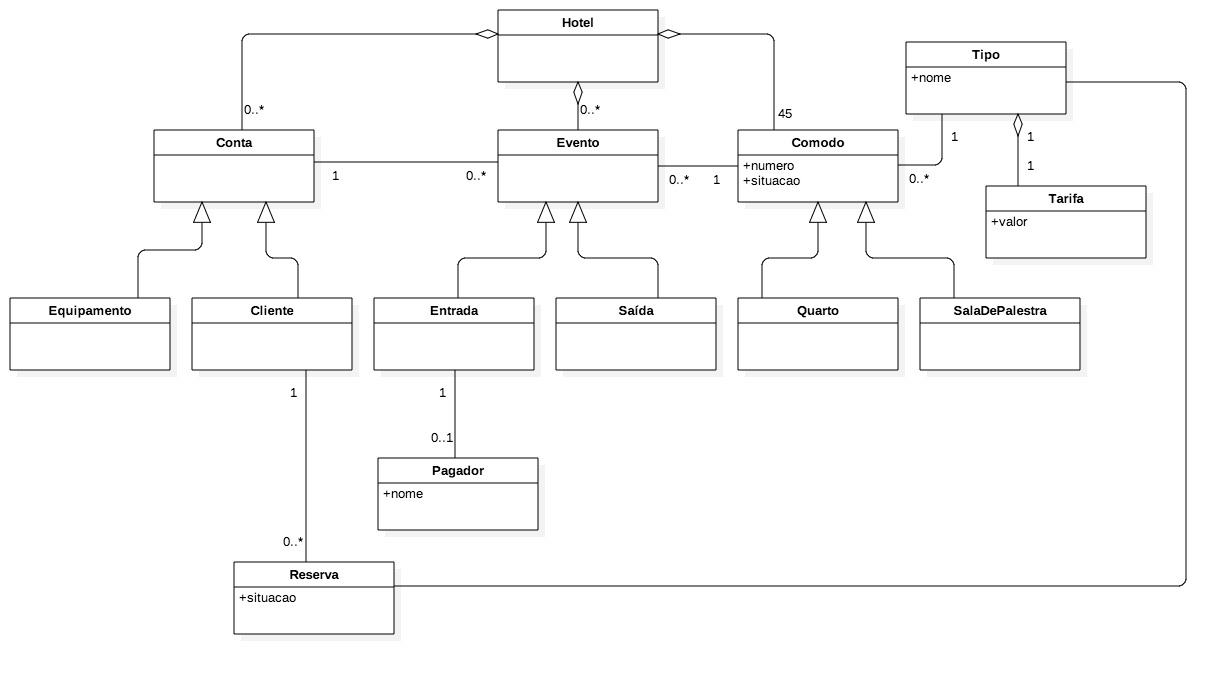
\includegraphics[width=0.92\textwidth]{./exercicios-hote-regina-diagrama-de-classes.jpg}
	\end{solution}

  \end{questions}

\end{document}
